%%This is a very basic article template.
%%There is just one section and two subsections.
\documentclass{article}
\usepackage{amsmath}
\usepackage{float}
\usepackage{graphicx}

\begin{document}


\section{Dense 3D Reconstruction using Robot Hand-Mounted Cameras}

This is a general sketch of an idea for reconstructing a dense 3D scene using a
hand-mounted depth camera.

\subsection{Problem}

Consider a robot that has a configuration space $C \subseteq \mathbf{R}^N$.
Mounted on one of the links of the robot is a depth sensor. The task is, given a
sequence of noisy configurations at each time step $\{q_1, q_2, \ldots,
q_T\}$, and a sequence of noisy sensor readings (point clouds) captured
simultaneously $\{Z_1, Z_2, \ldots, Z_T\}$, where $Z_i = \{x_1, \ldots, x_N\} \subseteq
\mathbf{R}^3$, reconstruct the true dense 3D geometry of the scene. 

\subsection{World Representation}

We will represent the world as a truncated signed distance function (TSDF). It
is defined as $D(x) : \mathbf{R}^3 \to \mathbf{R}$, and represents the (signed)
distance to the nearest obstacle in meters.

The gradient of the distance field $\nabla D : \mathbf{R}^3 \to \mathbf{R}^3$,
is clearly defined and easy to compute.

\subsection{General Approach}

We will iteratively build up the TSDF. $D_t$ is calculated by first estimating a
configuration of the robot $q^*_t$ which minimizes the squared error between the
sensor measurements $Z_t$ and the previous TSDF model $D_{t - 1}$. Then, the
sensor measurements are projected back into the world given $q^*_t$, and the
usual TSDF update is applied.

\begin{figure}
	\centering
	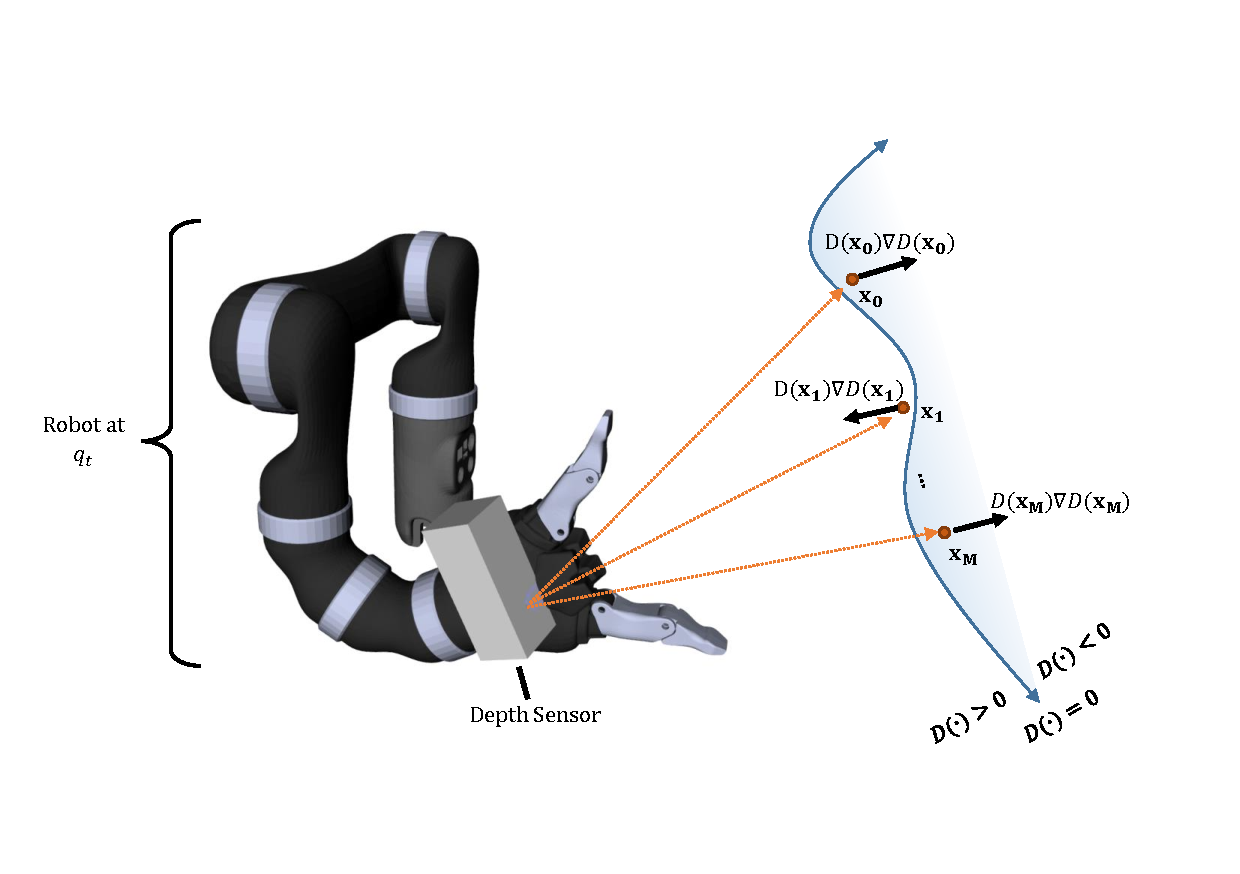
\includegraphics[width=1.0\textwidth]{img/robot_reconstruct.pdf}
	\caption{A diagram of the robot sensing a surface with a depth sensor. Rays
	from the depth sensor are shown as orange dotted lines. The point cloud
	$\{x_1, \ldots, x_M\}$ is used to determine the gradient of the distance field
	$\nabla D$ at each point.}
	\label{fig:robot}
\end{figure}

\subsection{Computing $q^*_t$}

We can compute $q^*_t$ by performing \textbf{gradient descent} in the
configuration space of the robot.  Define the \textbf{forward kinematics
function} $F(q_t, Z_t) : \mathbf{R}^3 \to \mathbf{R}^3$, which merely
transforms the point cloud $Z_t$ into the world frame, given configuration $q_t
\in C$. Call

$$ F_t = F(q_t, z_t) $$

Then, the objective function $h(q_t, D_{t-1}) : C \to \mathbf{R}$ is given by
the sum squared distances of all of the projected points in $F_t$:

$$ h(q_t, D_{t-1}) = \sum_{x \in F_t}\left(D_{t-1}(x)\right) ^2 $$

\subsubsection{Computing the Gradient}

Now, we want to find the partial differential of $h$ with respect to $q_t$:

\newcommand{\ddq}{\frac{\partial}{\partial q_t}}
\newcommand{\dxdq}{\frac{\partial x}{\partial q_t}}

\begin{align} 
\frac{\partial{h}}{\partial{q_t}} &= \ddq  \sum_{x \inF_t}\left(D_{t-1}(x)\right) ^2 
\\ &= \sum_{x \inF_t} \ddq \left(D_{t-1}(x)\right) ^2  
\\ &=\text{Making use of the chain rule? Since x is a function of~} q_t \ldots
\\ &= 2\sum_{x \in F_t} D_{t-1}(x) \dxdq \nabla D_{t-1}(x)
\end{align}

And, since $\dxdq$ is the change in $x$, a projected sensor point, with respect
to $q_t$, the configuration of the robot at time $t$, we have (with some
handwaving):

$$ \dxdq = \mathbf{J}_x \in \mathbf{R}^{3 \times N}$$

Where $\mathbf{J}_x$ is the serial manipulator Jacobian computed for the point
$x$, as though it were rigidly attached to the manipulator by the ray connecting
$x$ to the sensor. (This will make more sense with a diagram).

And so:

$$ \frac{\partial{h}}{\partial{q_t}} = 2\sum_{x \in F_t} D_{t-1}(x)
{\mathbf{J}_x}^{\text{T}} \nabla D_{t-1}(x) $$

\noindent We will call this quantity $\nabla h(q_t)$. It has a nice physical
interpretation: imageine all the points in the point cloud are attached rigidly
to the robot manipulator on rods. At then end of each rod $x$, apply a force
$D_{t - 1}(x) \nabla D_{t -1} (x)$. The resulting torque on the robot's joints
is proportional to $\nabla h(q_t)$ by a factor of 2 (Fig. \ref{fig:robot}).

\subsubsection{Gradient Descent}

Now, we just follow the update rule, setting ${q_t}^{(0)} = q_t$:

$$ {q_t}^{(i + 1)} = {q_t}^{(i)} - \lambda \nabla h(q_t^{(i)}) $$

\noindent Where $\lambda$ is a learning rate. We follow the gradient until
convergence, yielding $q^*_t$, treating the joint limits of the robot as a
constraint.


\end{document}
